
\section{Evaluation}
\label{sec:results}

In this section, we provide an evaluation of the \name system and the \tool UI analysis tool. We also report results from a small-scale user study, where we simulated a swapping attack on 15 study participants.

\myparagraph{Experiment setup} All experiments were performed on a laptop with a $3.2$ GHz quad-core Intel i5 CPU and $16$ GB memory running Ubuntu $16.10$ $64$-bit. We used Google Chrome version $61$ and JDK v$1.8$.

%\vspace{-5pt}
\subsection{\name Performance}
\label{sec:results:devicePerformance}

We evaluated the performance of our \device prototype using the following three metrics:

\begin{enumerate}
  \item \textbf{Page loading latency:} The elapsed time between the web page load and when the \device is ready to take input from the user. The \js code served by the remote server communicates with the \device and establishes a \tls using the \webusb API. The additional \tls messages and the \device processing introduce this delay only at the initial loading of the page. We measure the difference between the time when the \js code gets loaded into the browser and the time when the final \tls handshake message is sent.
  
  \item \textbf{Keystroke latency:} The added processing delay when the user presses a key. This time is due to the internal processing of the \device. We place the measurement at program point where the \texttt{USBHost} library starts capturing the keyboard event and at the program point the device sends the data via the \webusb interface to the browser.
  
  \item \textbf{Communication overhead.} The communication overhead between the \device and the remote server. As the \device establishes a separate \tls channel with the server, this adds data overhead to the standard HTTP communication between the browser and the remote server.
\end{enumerate}

We measured the page loading latency as $500$ ms (includes loading of the \webusb \js and establishment of the \tls channel between the \device and the remote server) and the keystroke latency as $5$ ms (both averaged over 500K iterations). These latencies are specific to the implementation architecture and the used boards, and that they can be reduced significantly using newer prototyping boards.\footnote{The master-slave $I^2C$ channel is limited to $1$ kHz. A Standalone implementation based on Arduino Genuino Zero, supported by the new version of the \webusb driver eliminates the $I^2C$ channel and reduces the latencies significantly.} 

Here, we emphasize that our solution is intended for user input integrity protection for specific security-critical operations. While a page loading latency of $500$ ms may be significant performance penalty for many web applications like online commerce in general, such a delay is insignificant for the types of operations like configuration of safety-critical devices that we focus on.

The communication overhead between the host system and the \device is very small. At the time of initialization, the \device and the remote server exchanges \tls handshake messages to establish the session. The handshake messages are $60$ bytes each. Each \tls message adds extra overhead of $80$ bytes (signature and announcement of next key). 

We also tested the performance overhead of the server-side processing. The server has to maintain an additional TLS connection ($TLS_2$) which has a small cost and match the parsed HTTP response with the received user input events which takes less than a microsecond. 
%The overhead of these extra steps is minor as the comparison of $265$ byte and $1$ kilobyte of data requires $60$ nanoseconds and $142$ nanoseconds respectively. This data is averaged over one million samples. 
From bandwidth point of view, the overhead of the second TLS channel is also small (this channel is only used to send the characters typed in by the user).

%\vspace{-5pt}
\subsection{\tool Evaluation} 
\label{sec:results:framework}

We evaluated our UI analysis tool implementation using two existing systems: PLC and home automation controller. The PLC system we used was ControlByWeb \emph{x600m}~\cite{controlbyweb} I/O server and we tested six separate configuration web pages for it. The home automation system we used is called home-assistant~\cite{ha} and we tested two different configuration pages for it. We wrote UI specifications these pages and the fed the specifications to our tool implementation. The tool produced groups of interchangeable user input fields that we the manually verified to be correct. Table~\ref{tab:evaluation} and~\ref{tab:evaluation2} provide the details of this evaluation, including specifications for tested UIs and reported swappable elements. Based on this evaluation, we make two conclusions. The first is that our tool is able to process configuration UIs of existing, commercially-available safety-critical systems. The second is that many such UIs have swappable user input fields that need protection provided by our labeling scheme.

\begin{table}[t]
\centering
\small
\caption[\tool user interface processing time]{\textbf{\tool user interface processing time.} We tested the processing time of our UI analysis tool on the web pages from the x600m PLC server, the home automation system and bitcoin wallets. All the measurements where conducted over 500K iterations.}
\begin{tabular}{lccc}
\toprule
\textbf{Web page} & \textbf{\#Fields} &\textbf{Processing time (ms.)} & \textbf{SD}\\ \hline
\multicolumn{4}{c}{x600m Web PLC} \\ \midrule
Register configuration & $6$ & $1.654$ & $0.0131$\\ 
Counter configuration & $7$ & $0.771$ & $0.0089$\\ 
Event configuration & $8$ & $0.622$ & $0.0085$\\ 
Action configuration & $5$ & $1.241$ & $0.0111$\\ 
Supply voltage & $4$ & $0.673$ & $0.0099$\\ 
Calender configuration & $11$ & $0.713$ & $0.0105$\\ \midrule
\multicolumn{4}{c}{Home automation} \\ \midrule
Home configuration & $6$ & $0.016$ & $0.0018$\\ 
Room configuration & $5$ & $0.012$ & $0.0015$\\ 
\hline
\multicolumn{4}{c}{Bitcoin wallet} \\ \midrule
Send Bitcoin & $4$ & $0.9$ & $0.024$\\ 
\bottomrule
\end{tabular}


\label{tab:frameworkPerformance}
\end{table}


Additionally, we tested our UI analysis tool on user interfaces of other PLC controllers, home automation systems, medical device control, personal data management and online banking. Again, we wrote specifications for these user interfaces and processed them through our tool that founds swappable input elements in many of the tested user interfaces. We mined around $35$ different text fields from $4$ different application types. We list our findings in Table~\ref{tab:inputFields}. We enumerate the user input fields in each page, their specifications that we manually created (including types and constraints) and the output of the tool that is grouping of swappable fields. We verified each output of the tool manually. We observe that in some cases the tool outputs as ``swappable'' input fields that can, in fact, be easily detected at the server. For example `start date' and `end date' are not swappable as the former has to be less than the later. This is an example of a case, where both fields are specified correctly, but their relationship imposes additional constraints that can be checked by the server. For such type of fields, the developers can exclude them from the input specification.

\begin{table}[!htpb]
\centering
\caption[\tool evaluation 1]{\textbf{\tool evaluation 1.} We tested our implementation of the UI analysis tool on `ControlByWeb x600m' industrial I/O server Web pages column shows the configuration pages that we tested. We list types and formats for each user input field in the tested pages, and also list those input fields that are swappable.}
\resizebox{\textwidth}{!}{
\begin{tabular}{llccp{2.4cm}}
\toprule
\textbf{Web pages} & \textbf{Fields} & \textbf{Type} & \textbf{Length/value constraint} &\textbf{Swappable fields} \\
\midrule
\multicolumn{5}{c}{\bfseries Web PLC configuration forms} \\
\hline
 & Name & \String& $[min=1, max=20]$ & Name \\  
 & Description & \String& $[min=0, max=60]$ & Description \\  
Register & Type & \integer& $[min=1, max=5]$ & Units \\\cline{5-5}
configuration & Units & \String& $[min=1, max=5]$ & Decimal place \\  
 & Decimal places & \integer& $[min=0, max=5]$ & Initial  \\  
 & Initial Value & \integer& $[min=0, max=999999]$ & Type\\

\midrule
 & Device & \radio & \{\texttt{on}, \texttt{off}\} & Name \\ 
 & Device counter number & \integer& $[min=0, max=50]$ & Description\\ \cline{5-5}
 & Name & \String & $[min=1, max=20]$ & Device counter number\\
Counter & Description & \String & $[min=0, max=60]$ & Decimal places\\
configuration & Decimal places & \integer & $[min=0, max=5]$ & Debounce \\
 & Debounce & \integer & $[min=0, max=9999]$ & Edge\\ 
 & Edge & \integer & $[min=0, max=6]$ & \\
\midrule

& Name & \String & $[min=1, max=20]$ & Name\\
 & Description & \String & $[min=0, max=60]$ & Description \\ 
 & Type & \menu & \{\texttt{int}, \texttt{float}, \texttt{boolean}, \texttt{constant}\}& \\ 
Event & I/O & \menu & \{available IO\} &\\ 
configuration & Event group & \menu & \{available Groups\} &\\ 
 & Condition & \menu & \{\texttt{On}, \texttt{Off}, \texttt{Equals}, \texttt{Change state}\}&\\ 
 & Eval on powerup & \radio & \{\texttt{yes}, \texttt{no}\} &\\ 
 & Duration & \integer & $[min=0, max=9999]$ &\\ 
\midrule

 & Name & \String & $[min=1, max=20]$ &Name\\ 
 & Description & \String & $[min=0, max=60]$  &Description \\ 
Action & Event source & \menu & \{available events\} &\\ 
configuration & Type & \menu & \{\texttt{On}, \texttt{Off}, \texttt{Toggle},\ldots\} &\\ 
 & Relay & \menu & \{Available relays\}&\\ 
\midrule

 & Name & \String & $[min=1, max=20]$ &Name \\ 
Supply & Description & \String &$[min=0, max=60]$ & Description \\ 
voltage & Decimal places & \integer & $[min=0, max=5]$ &\\ 
 & Device & \menu & \{Available devices\} &\\
\midrule

 & Name & \String & $[min=1, max=20]$ &Name  \\
 & Description & \String & $[min=0, max=60]$ & Description \\ \cline{5-5}
 & Event group & \integer & $[min=0, max=5]$ & Start date  \\ 
 & Start date & \Date & $[min=01/01/2007, max=31/12/2029]$ & Stop date \\ \cline{5-5}
Calender & Stop date & \Date & $[min=01/01/2007, max=31/12/2029]$ & Start time  \\ 
configuration & Start time & \Time &  $[min=00:00, max=23:59]$ & Stop time \\ \cline{5-5}
 & Stop time & \Time &   $[min=00:00, max=23:59]$ & Occurrence \\ 
 & All day & \radio & \{\texttt{on}, \texttt{off}\} & Repeat val\\ 
 & Repeat type & \menu & \{None, Secondly, Minutely, \ldots\} & \\ 
 & Repeat val & \integer & $[min=10, max=9999]$ &\\ 
 & Occurrences & \integer & $[min=0, max=999999]$ &\\ 
\bottomrule
\end{tabular}
}
\label{tab:evaluation}
\end{table}



\begin{table}[!htpb]
\centering
\caption[\tool evaluation]{\textbf{\tool evaluation 2.} Similar to Table~\ref{tab:evaluation}, we tested our implementation of the UI analysis tool on `home-assistant' home automation systems.}
\resizebox{\textwidth}{!}{
\begin{tabular}{llccp{2.4cm}}
\toprule
\textbf{Web pages} & \textbf{Fields} & \textbf{Type} & \textbf{Length/value constraint} &\textbf{Swappable fields} \\
\midrule
\multicolumn{5}{c}{\bfseries Web Home automation configuration forms} \\
\midrule

 & Room door lock & \radio & \rdelim\}{3}{25mm}[{\{\texttt{on}, \texttt{off}\}}] & Room door lock\\
 & Alarm & \radio & &Alarm \\ 
Home & Water lawn & \radio && Water lawn\\ 
configuration & Alarm time & \Time & $[min=00:00, max=23:59]$ &\\ 
 & Nest (thermostat) & \integer & $[min=16, max=25]$&\\ 
 & Sound selection & \menu & \{Available sounds\} &\\  
\midrule 

 & Table lamp & \radio & \rdelim\}{3}{25mm}[{\{\texttt{on}, \texttt{off}\}}] &Table lamp \\
Room & TV back light & \radio & &TV back light\\ 
configuration & Celling lights & \radio & &Celling lights \\ 
 & AC & \integer & $[min=16, max=25]$ &\\ 
 & Window shutter level & \integer & $[min=0, max=10]$ &\\
\bottomrule 
\end{tabular}
}
\label{tab:evaluation2}
\end{table}


\myparagraph{Example input fields}
Table~\ref{tab:inputFields} provides provides a listing of additional web UIs that we analyzed using the tool. The list includes web pages for online banking page, medical programmer device, PLC server and home automation system. The main purpose of this table is to provide examples (or templates) for the developer for the fields which they are likely encounter while analyzing with \tool. The table provides the names of the input fields along with their specifications, such as the regular expression and the length/value constraints, and whether some of the fields are mutually swappable or not.

We notice that some user input fields are strictly swappable only with another identical field.  Such as an arbitrary field is not swappable with bank account number such as \emph{IBAN} number due to the specific format (e.g., $[ISO 3166-1\ \text{IBAN code}] [0-9A-Z]^+$ with minimum and maximum length of $20$ and $30$ respectively).


%% -----------------
%% Additional UI specs table

\begin{table*}[!htpb]
\centering
%\footnotesize
\caption[Input field specifications]{\textbf{Input field specifications.} This table lists specifications (type, regular expression, length/value constraints) that we mined by analyzing various web pages (banking, medical, PLC, home automation). The swappable column denotes that the group of input fields with $\checkmark$ mark can be swapped with each other. Such as the current can be swapped with the frequency field.}
\resizebox{\textwidth}{!}{
\begin{tabular}{lp{0.5cm}cp{5cm}p{1cm}}
\toprule
\multicolumn{1}{c}{\textbf{Name}} &
\multicolumn{1}{c}{\textbf{Type}} &
\multicolumn{1}{c}{\textbf{Regular expression}} &
\multicolumn{1}{c}{\textbf{Length/value constraints}} & 
\multicolumn{1}{c}{\textbf{Swappable}}
\\
\hline
%\hline\hline
\multicolumn{5}{c}{\bfseries Personal information}\\
\cline{1-5}
Email & \rdelim\}{3}{15mm}[\String] & $(*)^+(@)[a-zA-Z0-9]^+(.)[a-z]^+$ & $[min = 5, max = *]$ & \\
%\cline{1-4}
Name & & $[a-zA-Z.]^+$ & $[min = 1, max = *]$ & \\
%\cline{1-4}
Address & & $[a-zA-Z0-9]^+$ & $[min=5, max=*]$ & \\
%\cline{1-4}
%\cline{1-4}\hline\hline

%\cline{1-4}
%\hline
\cline{1-5}
\multicolumn{5}{c}{\bfseries Medical parameters}\\
\cline{1-5}
Heartbeat & \rdelim\}{3}{15mm}[\integer] & \rdelim\}{3}{3mm}[] \multirow{3}{*}{$[0-9]^+$} & $[min=55,max=210]$ & \rdelim\}{4}{3mm}[$\checkmark$]\\
Blood pressure & & & $[min=80,max=150]$  &\\
Blood sugar (Fasting) & & & $[min=108, max=126]$  &\\
Body temperature & \float & $[0-9]^+((.)[0-9])^*$ & $[min=94,max=108]$ &\\

\cline{1-5}
%\cline{1-4}\hline\hline

\multicolumn{5}{c}{\bfseries Web-based PLC form~\cite{controlbyweb}}\\
\cline{1-5}
Analog Input(voltage) & \rdelim\}{2}{15mm}[\float] & \rdelim\}{2}{3mm}[] \multirow{2}{*}{$[0-9]^+((.)[0-9])^*$} & $[min=0,max=12]$ & \rdelim\}{8}{3mm}[$\checkmark$]\\
Current &  &  & $[min=300 (mA),max=2(A)]$  &\\

Thermocouple & \rdelim\}{6}{15mm}[\integer] & \rdelim\}{6}{3mm}[] \multirow{6}{*}{$[0-9]^+$} & $[min=-15,max=150]$ & \\
Frequency &  &  & $[min=0,max=500(Hz)]$ &\\
Logic repetition &  &  & $[min=0,max=9999]$ &\\
Event duration &  &  & $[min=0, max = 9999999999]$ &\\
Decimal places &  &  & $[min=0, max = 5]$ &\\
Initial value &  &  & $[min=0, max = 999999]$ &\\
%\cline{1-5}
Relay status & \rdelim\}{6}{15mm}[\radio] & \rdelim\}{6}{2mm}[] \multirow{6}{*}{$\{\texttt{On}, \texttt{Off}\}$} & \rdelim\}{6}{3mm}[]\multirow{6}{*}{$[min=0, max=1]$}  & \rdelim\}{6}{3mm}[$\checkmark$]\\
Thermocouple status & &  &   & \\
Thermocouple status &  &   & & \\
Energy slave status &  &  &  & \\
Input module status &  &  &  & \\
Thermostat status &  & & & \\
%\cline{1-5}
Logic start/end date & \Date & $[0-9]^+(/)[0-9]^+(/)[0-9]^+$ & $[min=1/1/2007, max=12/12/2029]$  & \\
%\cline{1-4}
Logic start/end time & \Time & $[0-9]^+(:)[0-9]^+$ & $[min=00:00:00, max=23:59:59]$  & \\
%\cline{1-4}
Logic Script & \rdelim\}{3}{15mm}[\String] & $(*)^+$ & valid controller script & \\
%\cline{1-4}
Module name &  & \rdelim\}{2}{5mm}[]\multirow{2}{*}{$[a-zA-Z0-9]^+$} & $[min=1,max=20]$ & \rdelim\}{2}{3mm}[$\checkmark$]\\
Description &  &  & $[min=0, max = 60]$ &\\

%\cline{1-4}
%\hline
\cline{1-5}
\multicolumn{5}{c}{\bfseries Web-based home automation}\\
\cline{1-5}
Room light toggle & \rdelim\}{4}{15mm}[\radio] & \rdelim\}{4}{2mm}[] \multirow{4}{*}{$$\{\texttt{On}, \texttt{Off}\}$$} & \rdelim\}{4}{3mm}[] \multirow{4}{*}{$[min=0, max=1]$}  & \rdelim\}{4}{3mm}[$\checkmark$]\\
Door lock toggle & & &  &\\
Alarm &  &  &   & \\
A/C &  &  &   & \\
%\cline{1-4}
Room temperature & \rdelim\}{2}{15mm}[\integer] & \rdelim\}{2}{5mm}[]\multirow{2}{*}{$[0-9]^+$} & $[min=6,max=25]$ & \\
%\cline{1-4}
Window shutter level &  &  & $[min=0,max=8]$ & \\
%\cline{1-4}
Alarm time & \Time & $[0-9]^+(:)[0-9]^+$ & $[min=00:00,max=23:59]$ & \\
%\cline{1-4}
\cline{1-5}
\multicolumn{5}{c}{\bfseries Web-based bitcoin wallet~\cite{bitgo,bitcoinwallet,coin,coinbase,blockchain}}\\
\cline{1-5}
\multirow{3}{*}{Address} & \rdelim\}{3}{15mm}[\String] & $[1][P2PKH]^+$ & \rdelim\}{3}{3mm}[]\multirow{3}{*}{$[min=34,max=42]$} & \\
&&$[1][P2SH]^+$&& \\
&&$[bc1][Bech32]^+$&& \\
BTC & \String & $[0-9]^+[.][0.9]^+$ & $[min=0.0,max=9999999999.0]$ & \\
Reference &\String& $[0-9a-zA-Z.-\ ]^*$& $[min=0,max=*]$ & \\

\cline{1-5}
\multicolumn{5}{c}{\bfseries Financial transaction, online banking} \\
\cline{1-5}
IBAN account no. & \String &$(ISO 3166-1\ \text{IBAN code}) [0-9A-Z]^+$ & $[min=20, max=30]$ & \\
%\cline{1-4}
Transaction amount. & \float & $(ISO 4217\ \text{currency code}) [0-9]^+((.)[0-9])^*$ & $[min=0, max=*]$  & \\

\bottomrule
\end{tabular}
}
\label{tab:inputFields}
\end{table*}


\myparagraph{Processing time} We measured the processing time of our tool. Table~\ref{tab:frameworkPerformance} shows our results: the processing time of one web page varies from 0.01 ms to 1.65 ms. The processing time depends on the number of states in the DFA constructed from the regular expression of the specification and the number of input fields. 

The time complexity of our UI analysis algorithm is exponential~\cite{Salomaa1997} ($\mathcal{O}(2^S)$) with respect to the number of states $S$ in the non-deterministic finite automaton (NFA) that is derived from the regular expression that is quadratic $\mathcal{O}(|F|^2)$ with respect to the number of input fields $|F|$. In practice, the analysis of tested UIs was very fast as i) the number of input fields is usually $6$ or less and ii) the DFAs from the specifications contain 2-3 states for most of the input fields.

%Algorithm~\ref{algo:makeGroup} is $\mathcal{O}(|F|^22^{|S|})$. Even though the running time is exponential in the number of states, most of the regular expressions of the text fields we encountered, are around 3-4, making the actual running time in the order of few milliseconds (refer Table~\ref{tab:frameworkPerformance} in Section~\ref{sec:results}).


%\vspace{-5pt}
\subsection{Preliminary User Study}
\label{sec:results:userStudy}

We also conducted a small-scale user study to understand whether the users can perform the proposed labeling correctly. 

\myparagraph{Recruitment} We recruited 15 study participants, aged 26-34, and all having a master's degree in computer science or related field.

\myparagraph{Procedure} We prepared a web page extracted from the ControlByWeb x600m I/O server. We passed this page through our \tool that annotated the page with the labeling instruction and converted drop-down menus to equivalent text fields. To simulate a swapping attack, we modified the page such that the description for the \texttt{`Relay temp 1'} and \texttt{`Relay temp 2'} fields were exchanged. The labeling instructions were unmodified.

We provided each study participant with an information sheet that provided brief background information on labeling and explained that the task is to configure a PLC device based on the provided instructions. We observed the study participants while they performed this task. %The figure in~\texttt{\url{https://goo.gl/oMFQBW}} 
Figure~\ref{fig:userStudyInstruction} shows the study UI and the information sheet.

\myparagraph{Results} Out of 15 participants, 7 noticed the inconsistency between the fields and labeling instructions in the UI, stopped the task, and report it to the study supervisor (\emph{Case 1} in Section~\ref{sec:securityAnalysis_IK}.2). Another 7 participants did not detect the UI inconsistency, but filled the input with correctly associated labels. The result is a correctly configured device (\emph{Case 2}). One study participants completed the labeling incorrectly and fell for the attack (\emph{Case 4}). The users reported that the additional labelling does not pose any significant effort. Additionally, none of the users made any mistakes while writing the labels in the text field along with the data. 

\myparagraph{Ethical considerations} Our user study did not collect any private information, such as email addresses or password. In such cases, our institution does not issue IRB approvals.

\myparagraph{Study discussion} In our user study, we provided brief instructions the participants as shown in see Figure~\ref{fig:userStudyInstruction}. This is in line with the primary usage of our system, where \name is used by trained professionals, who configure medical devices, industrial PLC systems and similar safety-critical devices. The secondary user group of our system is people like home automation system owners or cryptocurrency wallet users who have not received training for the task. Our study was not tailored for this scenario.


\begin{figure*}[t]
 \centering
 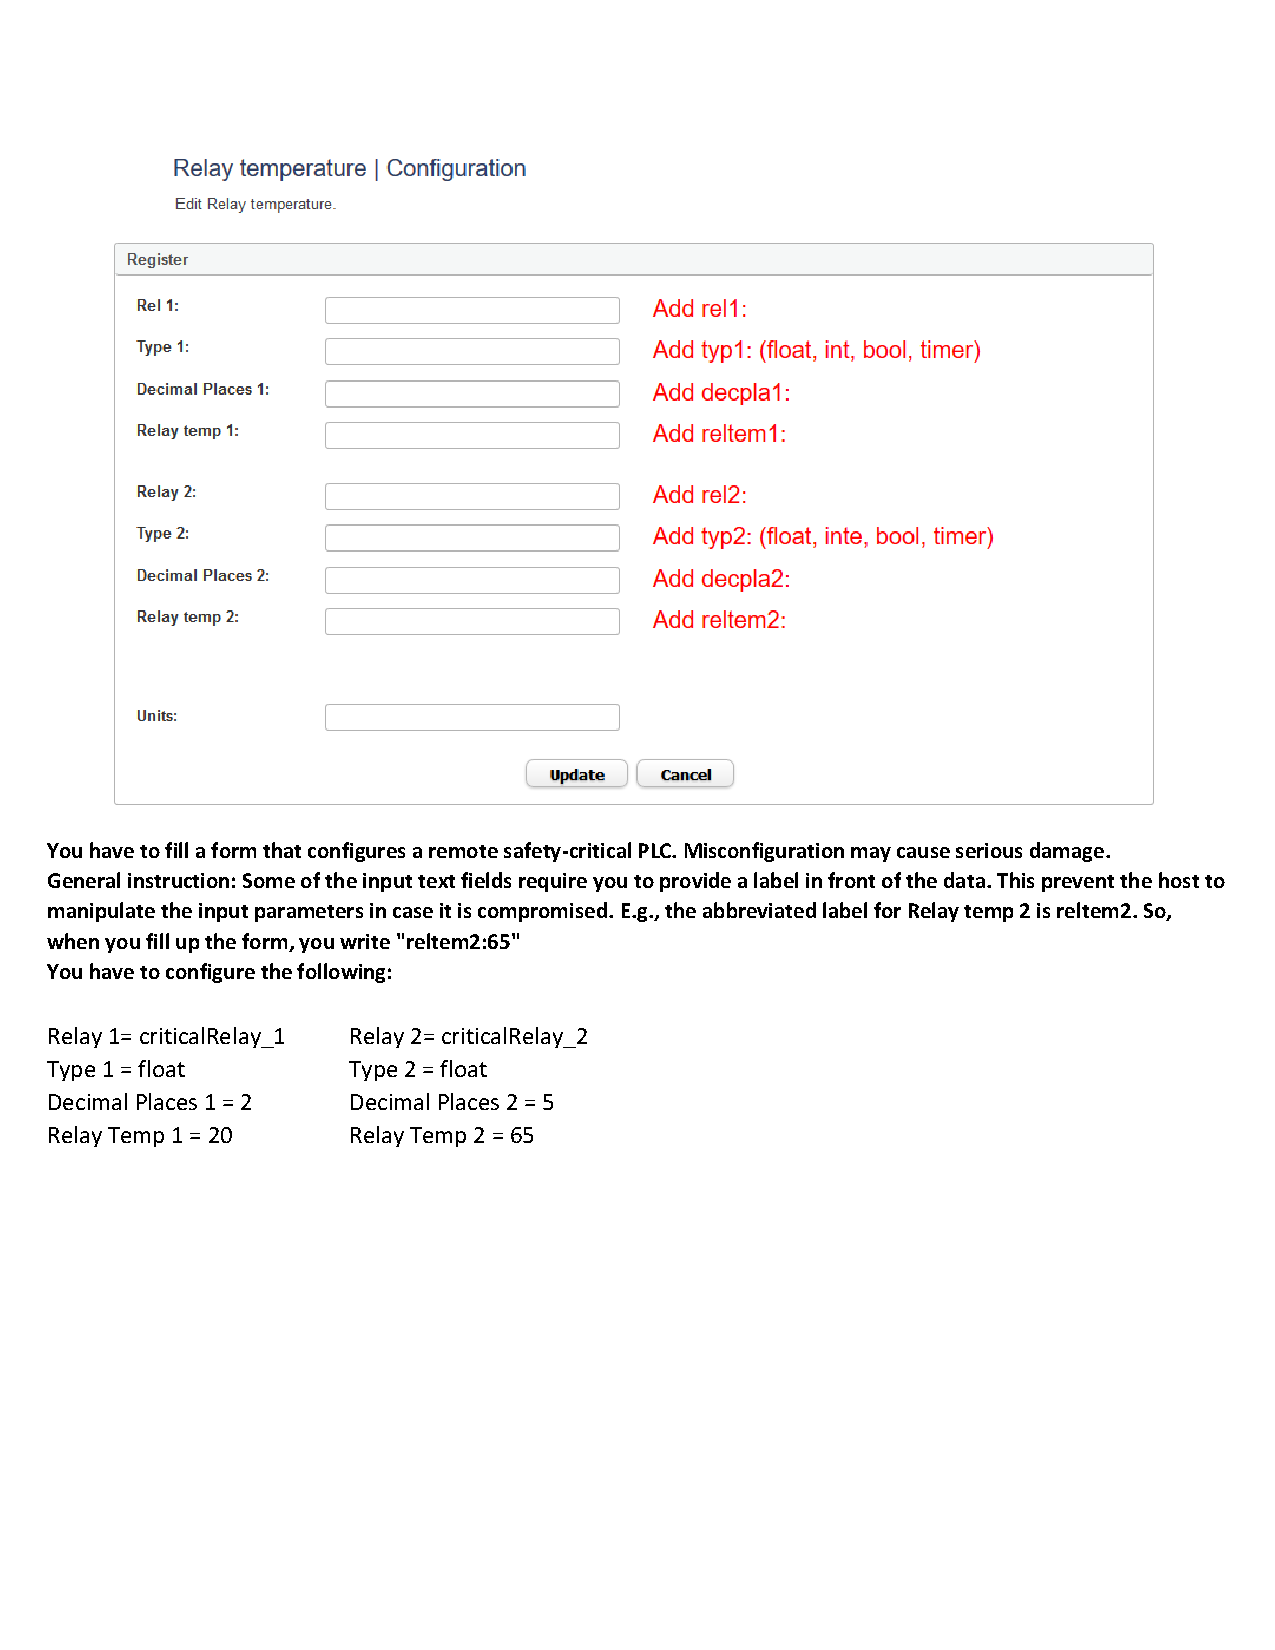
\includegraphics[trim={0 8cm 0 2cm}, clip,width=\linewidth]{chapters/IntegriKey/images/userStudy.pdf}
 \caption[User study instructions]{\textbf{User study instructions.} This figure shows the instruction sheet that was given to our user study participants.}
 \label{fig:userStudyInstruction}
\end{figure*}

%We got necessary permission from our institutes' ethics board for conduction the study. 

%\begin{table}[t]
%\centering
%\scriptsize
%\caption{\textbf{User study} .}
%\begin{tabular}{lccc}
%\hline
%\textbf{\#Participants} & \textbf{Errors made} &\textbf{\#Attack detected} & \textbf{\#Successful attack}\\ \hline
%$14$ & $0$ & $7$ & $1$\\ 
%\hline
%\end{tabular}
%\label{tab:userStudy}
%\end{table}


